%\RequirePackage[2020-02-02]{latexrelease}
\documentclass[12pt,onecolumn,aps,prb,preprint]{revtex4}   % style for Physical Review B and AJP are similar
\usepackage{amsmath}    % need for subequations
\usepackage{amssymb}
\usepackage{graphicx}
\usepackage{float}
\usepackage{svg}
\usepackage{listings}
\usepackage{subcaption}
\captionsetup{compatibility=false}
\newcommand{\dprime}{{\prime \prime}}
\newcommand{\beao}{\begin{eqnarray}}
\newcommand{\eeao}{\end{eqnarray}}
\newcommand{\mypm}{\mathbin{\mathpalette\@mypm\relax}}

\begin{document}

\title{Robotic Reconstruction of Islamic Calligraphy with Rotating Bezier Splines}
\author{Muhammad Umar Hassan, 2017-MS-MC-17}
%\includepdf{UETFormattedTitlePage.pdf}
\begin{abstract}
\label{Chapter:Abstract}
{
    Automated reconstruction of Islamic architectural calligraphy can save thousands of nobel and historic scripts all over the world from going extinct. One of the fundamental problems in such reconstruction tasks is the absence of a tool that can bridge the gap between artists and the machines (such as a robotic arms) by taking input as conventional calligraphy format and transform into a robot-program. Not just the reconstruction, even in this digital age, no such method exists that lets the artists generate new broad-edge scripts that can be reproduced mechanically. In this context, the research presented herein introduces a novel innovation in the conventional Bezier spline curves to use them to effectively answer the artistic requirements of copying or creating broad-edge calligraphy scripts and can directly produce data needed by the industrial robots. To demonstrate the effectiveness of our approach, two famous scripts are reproduced using the new splines and a comparison is made with the originals. Additionally, to establish how these splines can be used with machines, a robotic simulator is also discussed and the output analyzed both qualitatively and quantitatively. In addition to mechanized reconstruction Islamic calligraphy, the presented approach can also be used for generating calligraphy for virtual 3D models, e.g. in Metaverse, 3D documentation of non-reachable and ruined buildings and even OCR of islamic calligraphy scripts.
}
\end{abstract}

\maketitle
\tableofcontents
\input{03 - Introduction.tex}
\section{Understanding the Research Problem}
\label{Chapter:Problem Statement}
{
    \subsection{The Problem Statement}
    {
        The main problem is to devise a solution to use a robotic manipulator with a broad edge tool to create and copy Islamic calligraphy specimens. This problem can be divided in four main questions:
        \begin{itemize}
          \item How to copy and create broad-edge scripts in the computer?
          \item How to format the data in digital format to include most of the script information?
          \item How to convert the digital data into machine data to be used with actual manipulators?
          \item How accurate and robust is the proposed solution.
        \end{itemize}

        The first task would be to study the existing digital forms of Islamic calligraphy which are mainly based on glyphs and splines that form digital computer fonts. They carry the least information to reproduce the final ink-marks of the script. They don’t carry information about the machine movement. Conventional bezier splines could also solve the problem if they could either be translated into machine data or could somehow contain machine data within in the first place. This new method then needs to be tested and characterised. This is why a simulation solution would also be needed.

    }
    \subsection{The Proposed Solution}
    {
        As we discuss in section \ref{Chapter:Twisting Splines}, the first three questions of the research can be directly answered by one innovation in the conventional bezier splines. We discuss in detail how the twisting splines work but the main idea is to include a human artist in the process. The artist is given a computer interface that mimics a broad edge tool in the same fashion similar to most vector graphics editors that work well for round tip pens. The main strength of the innovation lies in the fact that though the artist may be oblivious to what they are actually producing, they actually are also feeding direct machine data information in the spline. The output is vector data; sum of a number of continuous step functions and can be considered directly as the end effector movement data.

        Once an editor for such splines is ready, the main challenge would be the characterization and testing of the proposed technique. Section \ref{Chapter:Twisting Splines} also shares some results and benchmarks of the twisting splines.

        To verify how well the splines work with a real manipulator, a $6$ DoF robotic manipulator would be needed. Section \ref{Chapter:Drogon} discusses such a simulator written specifically to test the splines. We can use the graphical and programmatic interface of the simulator to test and quantitatively analyze the rotating bezier splines with different configurations of a robot.
    }
}

\input{05 - Rotating Bezier Splines.tex}        % Twisting Bezier Splines
\section{Robotic Manipulator}
\label{Chapter:RoboticManipulator}
{
    \subsection{Functional Requirements of the Manipulator}
    {
        To fully test the twisting splines with a robot, a simple simulator was written as a desktop application. The following sections will now discuss a manipulator with six degrees of freedom used to test the splines. The details about working and design of the simulator are discussed in section \label{Chapter:Drogon} in Appendix 1. We now take a little diversion from the twisting splines to discuss the manipulator and then discuss their incorporation in the simulator in section \ref{Section:SimulatingRBS}.
    }
    \subsection{Functional Requirements of the Manipulator}
    {
        Typically, a robot is required to perform precise maneuvers with complete $6$ degrees of freedom of the end effector in both planar and curved planes. It is also required to provide at least one extra actuator to reduce singularities. In addition to position, the robot is also required to perform precise velocity and force controlled maneuvers. However, to use the test case of twisting bezier spline curves, not all of these functional requirements are forced. The manipulator has only six degrees of freedom and incorporates only a position control mechanism.
    }
    \subsection{Manipulator Representation}
    {
        Conventionally, the robot can be represented on a piece of paper using simple symbols and links as shown in Fig. \ref{FigConventionalRep}
        \begin{figure}[hb]
          \centering
          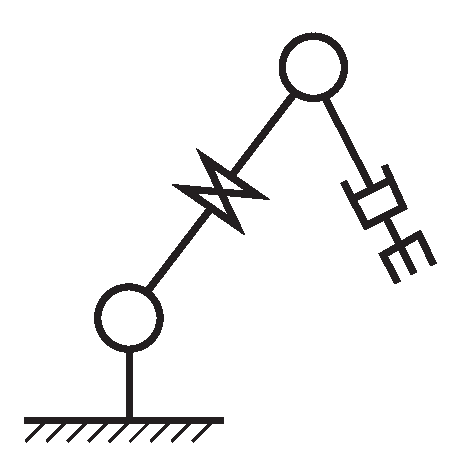
\includegraphics[width=0.5\textwidth]{../Images/RobotRep1.pdf}
          \caption{Conventional way of representing a manipulator. The circles show a rotation between the interconnected links on the plane of the paper. The cross symbol shows rotation on the link line. The square symbol is for prismatic joint. It represents change in length along the link line.}\label{FigConventionalRep}
        \end{figure}
        This kind of representation is clean and simple but doesn't give a complete view of the robot. Specially, with virtually zero link lengths, the visual representation can confuse someone new to the realm of robotic. Based on repeated experiments and to answer the weakness of contentional representation, we propose a new kind of representation that encapsulates the basic idea of representation with some features of a $D-H$ table. See Fig. \ref{FigMyRep}
        \begin{figure}
          \centering
          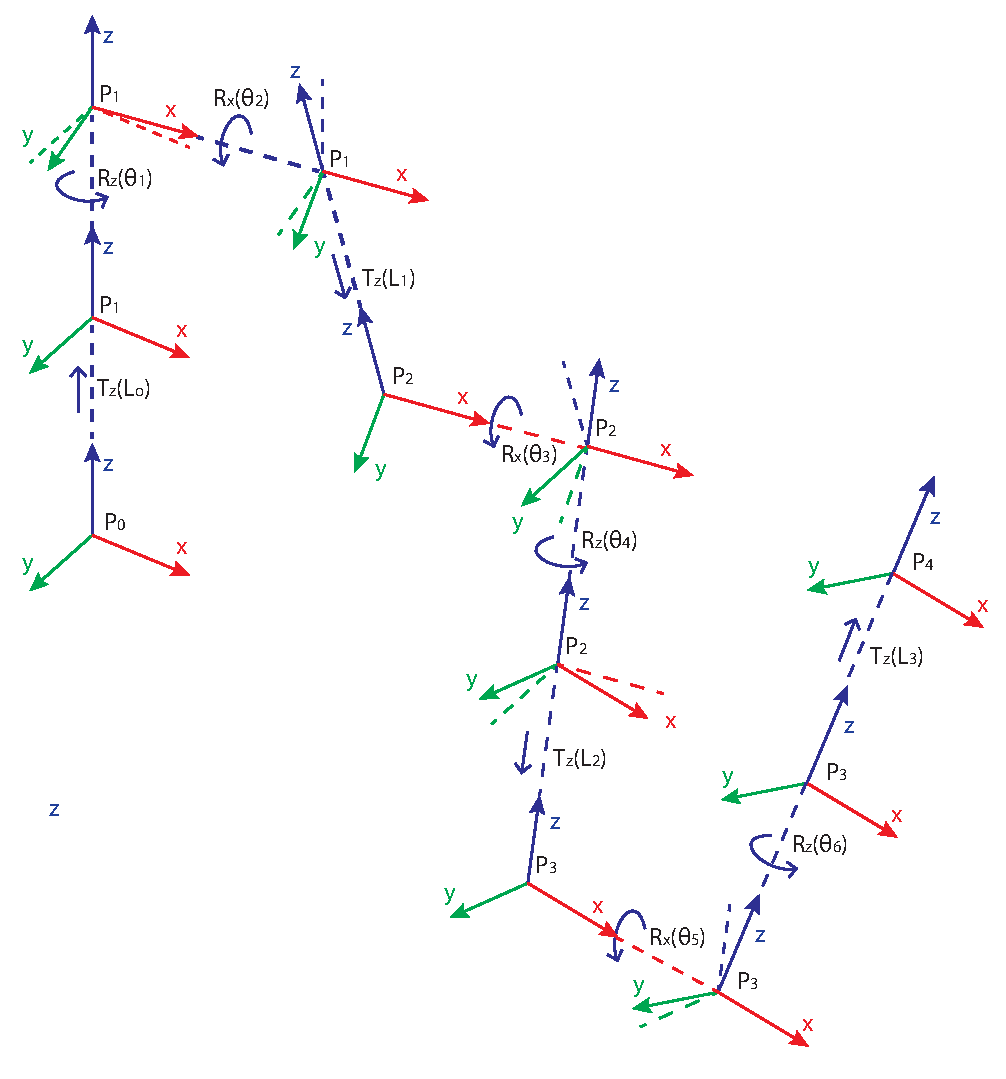
\includegraphics[width=0.8\textwidth]{../Images/MyRep.pdf}
          \caption{An example of \texttt{transformation frames} representation. This representation shows how a reference frame is linked to the previous using two basic transformation functions, $T_n$ and $R_n$ where n is the axis along or about which the transformation is performed. The schematic is drawn in the direction of $F0$ to $F_N$ ($N$ being the last frame) but can also be interpreted in reverse direction. One can easily see which transformations are required to convert one frame of reference to the other. One only needs to take one thing in account. When going in forward direction, all the transformations are applied as they are but while going back, each successive transformation is taken as inverse. For example, frame $F5$ can be achieved from frame $F3$ by applying two successive transformations: translation along $x$ of magnitude $L1$ and rotation about $x$ of magnitude $\theta_3$. However, to go to frame $F3$ from frame $F5$, one needs to apply two successive transformations: rotation about $x$ of magnitude $-\theta_3$ and translation along \texttt{x} of magnitude $-L1$. It should be noted that if a transformation changes the origin of the frame, the next frame has a different point shown at the center. This point is defined in the base frame.
          } \label{FigMyRep}
        \end{figure}

        Interestingly, this representation can't only represent physical manipulators, it can also represent abstract transformations. See Fig. \ref{FigEulerRep} which represents a target $P_t$ being represented as $z-x-z$ euler angles.

        \begin{figure}
          \centering
          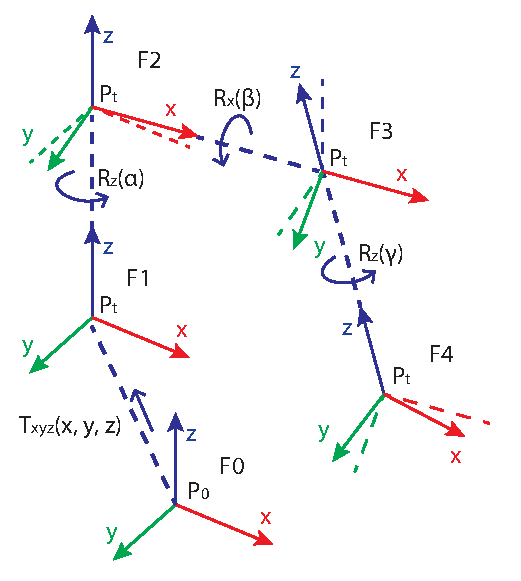
\includegraphics[width=0.6\textwidth]{../Images/EulerANgles.pdf}
          \caption{Three successive rotation $z-x-z$ and similar orders are call \texttt{Euler Angles Transformations}. A base Frame $F0$ is transformed though three translations and three euler rotations. This way, one can easily represent a target point to the robot which would have three extra components than $x$, $y$ and $z$; $\alpha$, $\beta$a and $\gamma$.
          } \label{FigEulerRep}
        \end{figure}

        Now, if one represents both target and the manipulator representation in a solved state, a closed loop representation can be formed which becomes extremely convenient in inverse kinematics. See Fig. \ref{FigCompleteRep} which exemplifies a closed loop \texttt{transformation frames} representation. It should be quite clear that once a closed loop is constructed, one can make transformations in any direction.

        \begin{figure}
          \centering
          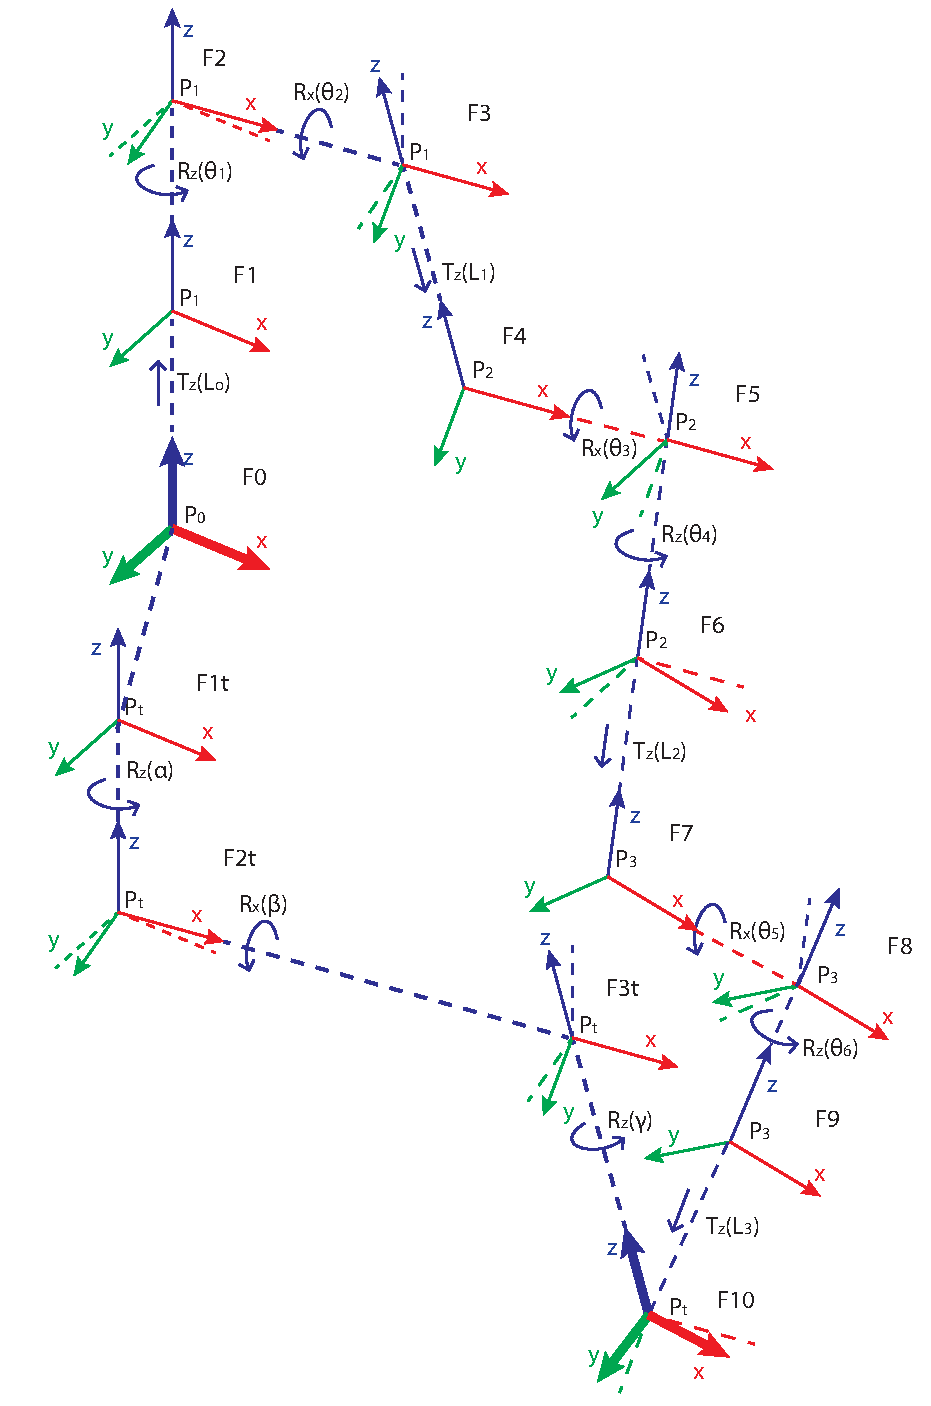
\includegraphics[width=0.8\textwidth]{../Images/CompleteRep.pdf}
          \caption{A manipulator along with a target represented in \texttt{transformation frames} representation. $F0$ corresponds to the base frame, $F0, F1, F2 ...$ represent the forward direction of the manipulator and $Ft0, Ft1, Ft2 ...$ represent the forward direction of the target. Both chains of transformations lead to a common reference frame eventually, the target frame of reference, or the end-effector frame of reference, $Ft$.
          } \label{FigCompleteRep}
        \end{figure}

        It is interesting to see that while doing a complete cycle transformation, one virtually transforms a frame through nothing! Also, if a $N-1$ frame transformation is applied in a $N$ frame closed loop, one can identify one last transformation quite easily by comparing the initial and the final frames. This method is called \texttt{Known Error Propagation} and will be used extensively in the inverse kinematics.

        Last, but not the least, of the usages of a closed loop representation is that some transformations can be skipped/swapped safely in order to simplify the loop. This can lead to finding further more unknown parameters using \texttt{Known Error Propagation}.

    }
    \subsection{Selecting a Configuration}
    {
        The configuration selected for this project is widely used by other engineers but the main inspiration behind choosing this configuration was a B.Sc. final year project of the \emph{Mechanical Engineering Department of U.E.T} of the batch $12$' with title, 'Design and Implementation of a $6$DoF Spot Welding Robot'. The project report presents a solution and describes all the forward and inverse kinematics. And all this, without using a regular transformation matrix! The effort in the current project takes some inspiration from the previous one and also elaborates not only the faults and issues with the previous but also the effectiveness of using transformation matrices.

        See Fig. \ref{FigCompleteRep} which represents this manipulator. It has six rotating actuators linked together with four links.
    }
    \subsection{Mathematical Modelling}
    {
        Using the new representation, properties of homogenous transformation matrices and basic highschool trigonometry, I was able to calculate \cite{bib21} the unique and redundant solutions for the spherical manipulator. The manipulator has two primary solutions: different joint positions yield the same end effector position and orientation. Connected to both solutions, are $4$ more secondary solutions which effect only the motor angles not the link locations.

        Finding out the mathematical equations is one job, verification is another. While dealing with three dimensional realm on a two dimensional paper, one can the solution but making small human errors on the way. It is quite easy to confuse the directions of rotations in a reference frames, resulting in typical errors which can be mitigated by some hit-and-trial of a few operations; adding or subtracting integral multiples of $\frac{\pi}{2}$ from the angles, inverting the length signs, inverting the angle directions. This can be done easily only if a representation tool is build alongside the robot modeling.
    }

    \subsection{Inverse and Forward Kinematics}
    {
        Some of the motor angles are quite obvious. See the series of hand-sketched figures labelled with mask Fig. \texttt{RDn} in the subsequent pages which demonstrate how an inverse kinematic solution was discovered for this robot.
    }

    \subsection{Incorporating the twisting bezier splines} \label{Section:SimulatingRBS}
    {
        Using the same model of the spline model, the simulator first rasterizes the whole spline and then transforms the two dimensional points onto a plannar surface simulated on a user desired position in the workspace. Then it creates a pseudo machine code to mimic the tool changes required before each stroke and the transformed rasterized points are directly considered as G-Codes for the manipulator. Once computed it starts implementing the program.

        For the sake of analysis, in parallel, the end effector orientation is captured continuously to construct an ink mark with each sweep of the tool. The reproduced image is then used for analysis. The results of such a comparison can be seen in Table \ref{Table:MachineDataMetrices}. The value indicate that the robot very closely reproduces the given spline thus verifying the thesis of the research.

        \begin{table}[ht]
        \centering
        \resizebox{\textwidth}{!}{\begin{tabular}{| p{0.3\linewidth} | p{0.3\linewidth} |  p{0.2\linewidth} |  p{0.2\linewidth} |}
          \hline
          & \textbf{Reference} & \textbf{Coverage} & \textbf{Extra} \\
          \hline
          \multicolumn{4}{|l|}{\textbf{Nastaleeq}}\\
          \hline
          Rotating Bazier Spline & Original Image & 95.8\% & 5.4\% \\
          \hline
          Machined Output & Original Image & 96.7\% & 7.0\% \\
          \hline
          Machined Output & Rasterized Image & 96.7\% & 4.3\% \\
          \hline
          \multicolumn{4}{|l|}{\textbf{Thuluth}}\\
          \hline
          Rotating Bazier Spline & Original Image & 93.4\% & 2.8\% \\
          \hline
          Machined Output & Original Image & 95.0\% & 3.4\% \\
          \hline
          Machined Output & Rasterized Image & 97.8\% & 4.4\% \\
          \hline
        \end{tabular}}
        \caption{Benchmark of the mathematical accuracy of the twisting bezier spline curves with a simulated manipulator}
        \label{Table:MachineDataMetrices}
        \end{table}
    }
}
\clearpage         % Robotic Manipulatorv
\section{Gregor -- The Twisting Bezier Spline Editor}\label{Chapter:Gregor}
\subsection{Introduction}
{
    The twisting Bezier splines may well mathematically be able to quite accurately contain most of the information required to replicate a calligraphy artwork but will hardly be practically useful without a tool strong enough to enable an artist to effectively trace an existing or create a new calligraphy specimen. Now, making such a tool was in itself an entire software engineering project and could not easily fit in the scope of the on going work. However with this link missing, in would have been impossible to quantitatively test and benchmark the performance of the other tools. So the least that could actually be done would be to layout the bare minimum user requirements and start writing the tool. The coding work was only as linear as any other software project which relies on ambiguous and equivocal requirements. Meaning that once the first version of the software had been built, the software had to be taken back to development many times after tests with real artists. Some features were added later to fulfil the necessity that was felt during the trial while others which were initially considered to be cardinal to working of the application.

    The name ``Gregor'' is taken from a character of George R. R. Martin's legendary novel\cite{bib19} series Game of thrones. He is one of his kind; not the fastest fighter there is but is strong and every blow of his sword is effective.

    Once the application had been developed, came another step which is often forgotten and considered dispensable usually by most developers; documenting the code and the usage. Documentation of the code and a user manual is the only thing that turns an application into a software. As said earlier, keeping in view the scope of the project, the documentation too had to be limited to contain only the most critical parts. This chapter may serve as the user manual of the software. The user guide includes:
    \begin{itemize}
      \item describing how the application should be used normally,
      \item the user interface,
      \item keyboard shortcuts,
      \item saving and loading data, and
      \item introduction to analysis tools.
    \end{itemize}
    While the coding manual includes:
    \begin{itemize}
      \item general code organization,
      \item architecture and functionality of the most important parts of the code, and
      \item the relationships between most significant entities.
    \end{itemize}
    Additionally, some snippets of the code are also included in the printed appendix and in addition to uploading the whole code as a GitHub repository \cite{bib20}, it can be found in Appendix \ref{Appendix:sourceCode} which is a digital copy that can be accessed by most computers and smart-phones.
}
\subsection{Requirements}
{
    The most fundamental user requirements are very simple.
    \begin{itemize}
      \item
      {
        The most fundamental requirement was that the tool be able to let the user graphically draw a rotating bezier spline. It was not only convenient but also logical to make the editing sequence similar to other vector editing software. This will make the transfer easier for people who already have some experience in other applications.
      }
      \item
      {
        The application must be able to save and load the edited work using a data file.
      }
      \item
      {
        The user should be able to drag and zoom the view port using the mouse cursor and keyboard shortcuts.
      }
      \item
      {
        There should be a provision to load images into the workspace so that they can be traced.
      }
    \end{itemize}
}
\subsection{Overview of the implementation}
{
    Gregor provides the minimal functionality to work with twisting bezier splines. Additionally, many of the secondary features were implemented to fulfil the needs of actual artists who found the basic interface too wanting. Microsoft .Net framework was chosen to construct the GUI application mainly because it supports writing code in Microsoft Visual C Sharp (C\#) and because all the intended features like mouse and keyboard interactions and graphics are easy to implement in it. Gregor can create, modify, import and save twisting splines. it mainly consists of a single \emph{Windows Form} that hosts the basic editing and viewing controls and an interactive workspace. The workspace is a virtual page that can be zoomed into and panned around using the cursor and keyboard shortcuts. One can change the viewing modes of the workspace to better suite the editing needs. One can choose to display or hide certain anchors, ink-marks, curvature spline, and change the appearance of a twisting spline. To assist the user, Gregor also allows to import and scale images that can be used to trace twisting bezier splines.
    
    See Appendix \ref{Appendix:Gregor} that describes the interface, enlists the features and describes the usage of most important parts of the application.
}
\clearpage
\input{08 - Drogon.tex}
\section{Conclusion}
\label{Chapter:Conclusion}
{
    The twisting Bezier spline curves very closely mimic the ink mark of broad edge tools thus creating very accurate calligraphy scripts as seen in Figure \ref{Image:spline_prev}. With most of broad edge scripts, on an average, they give more than 95\% coverage of the reference image an less than 5\% overdraw. This has now been verified by comparing them with original calligraphy specimens as well as after simulating the output of a robotic manipulator.

    \begin{figure}
      \centering
      
\includegraphics[width=0.7\textwidth]{../Images/rotating bezier splines preview.pdf}
      \caption{A preview of the calligraphy produced using the rotating bezier splines.
      } \label{Image:spline_prev}
    \end{figure}

    With tools created as a by-product of this research, an artist can not only trace existing calligraphy scripts, but also create and modify new ones with a very lean learning curve. The ease of use of the tools created for the tast assures that the focus of the artist is more on the art itself than the caveats of the software solution.

    Where the accuracy of the splines has been characterised and ease of use has been demonstrated, there still are a lot of unexplored areas that require more research. As discussed in section \ref{ExplorationPoints1}, one can pack the tool inclination and normal pressure information into the rotating splines. One can also choose to implement other kinds of manipulators and actuators to test the performance of the splines in the simulator. Last but not the least, since the simulator can emulate a pseudo robot, it can also be modified to be used as a live controller for a real robotic manipulator.

    While this thesis puts together the results of some crucial tests to establish the usefulness of rotating splines, the final verdict will still be given by the community that takes the work forward in more scenarios and conditions.
}
\clearpage 
\input{10 - Bibliography.tex}
@@ -1,465 +0,0 @@
\appendix
\section{Tables}\label{Appendix:Tables}
\subsubsection{Gregor -- Keyboard Shorcuts}
{
\begin{table}[ht]
    \centering
    \resizebox{\textwidth}{!}{\begin{tabular}{| p{0.35\linewidth} | p{0.6\linewidth} |}
      \hline
      % after \\: \hline or \cline{col1-col2} \cline{col3-col4} ...
      Key & Action \\
      \hline
      \multicolumn{2}{|c|}{The File Menu} \\
      \hline
      Ctrl + O & Open an existing document \\
      Ctrl + S & Save the document to the last selected file or a new file if no previous file is associated. \\
      Ctrl + Shift + S & Save the data in a new file \\
      Ctrl + I & Import spline data from file \\
      Ctrl + E & Open up the export menu \\
      Shift + Del  & Clear the workspace \\
      Alt + F4 & Close the application \\
      \hline
      \multicolumn{2}{|c|}{The View Menu} \\
      \hline
      Ctrl + 4 & Combined Mode; Shows both ink and curves \\
      Ctrl + 5 & Ink Only Mode; Shows Only the ink marks and hides the curve alogwith the handles \\
      Ctrl + 6 & Splines Mode. Hides the ink marks \\
      Ctrl + G & Toggle the visibility of the grid \\
      Ctrl + Shift B & Toggle the visibility of the background images \\
      \hline
      \multicolumn{2}{|c|}{The Edit Menu} \\
      \hline
      Ctrl + 1 & Toggles the splines anchor centers \\
      Ctrl + 2 & Toggles the splines curvature handles \\
      Ctrl + 3 & Toggles the rotation handles \\
      Ctrl + V & Toggles the action of mouse left click between adding the anchor and dragging the workspace. \\
      \hline
      \multicolumn{2}{|c|}{Help}\\
      \hline
      F1 & Shows quick help \\
      F2 & Opens up the project Git.\\
      \hline
    \end{tabular}}
    \label{Table:Keyboardshortcuts}
    \end{table}
}
\clearpage
\section{Source Code}\label{Appendix:sourceCode}
{
    \clearpage
}
\section{Code Snippets}\label{Appendix:CodeSnippets}
{
\begin{lstlisting}[language=XML]
//Sample code of a rotating Bezier spline that will render the Urdu letter Aa'en in Nastaleeq.
<spline>
    <FlatTipWidth>150</FlatTipWidth>
    <Color>-5658199</Color>
    <anchor>
      <rotationoffset>0</rotationoffset>
      <P>-198.3791, 452.6993</P>
      <C1>-131.6351, 572.4461</C1>
      <C2>-265.1234, 332.9534</C2>
      <R1>-148.3791, 452.6993</R1>
    </anchor>
    <anchor>
      <rotationoffset>0</rotationoffset>
      <P>-296.5323, 156.2775</P>
      <C1>-439.8357, 254.4304</C1>
      <C2>-119.5302, 35.04326</C2>
      <R1>-246.5322, 156.2775</R1>
    </anchor>
    <anchor>
      <rotationoffset>0</rotationoffset>
      <P>25.40986, 374.1774</P>
      <C1>-47.22344, 262.2825</C1>
      <C2>98.04301, 486.0714</C2>
      <R1>75.40986, 374.1774</R1>
    </anchor>
    <anchor>
      <rotationoffset>0</rotationoffset>
      <P>-233.7143, -183.332</P>
      <C1>-208.1945, -28.25013</C1>
      <C2>-274.7982, -432.9961</C2>
      <R1>-183.7143, -183.332</R1>
    </anchor>
    <anchor>
      <rotationoffset>0</rotationoffset>
      <P>315.9428, -517.0526</P>
      <C1>95.77186, -679.5702</C1>
      <C2>435.6645, -428.6809</C2>
      <R1>365.9427, -517.0526</R1>
    </anchor>
    <anchor>
      <rotationoffset>0</rotationoffset>
      <P>441.5787, -144.0708</P>
      <C1>388.576, -277.5591</C1>
      <C2>494.5813, -10.58265</C2>
      <R1>491.5787, -144.0708</R1>
    </anchor>
  </spline>
\end{lstlisting}
}
\section{Images}
{

\begin{figure}[H]
  \centering
  \includegraphics[width=0.8\textwidth]{../Images/Nastaleeq_Ink.pdf}
  \caption
  {
      Nastaleeq sample by Gohar Qalam. (a) Original calligraphy photo. (b) Original photo processed for analysis. (c) Traced rotating bezier spline ink. (d) Difference between (b) and (c). The red pixel indicate the portions that are missing in (c) but are present in (b) and the blue ones show the missing pixels in (b) but are present in (c).
  }
\end{figure}

\begin{figure}[H]
  \centering
  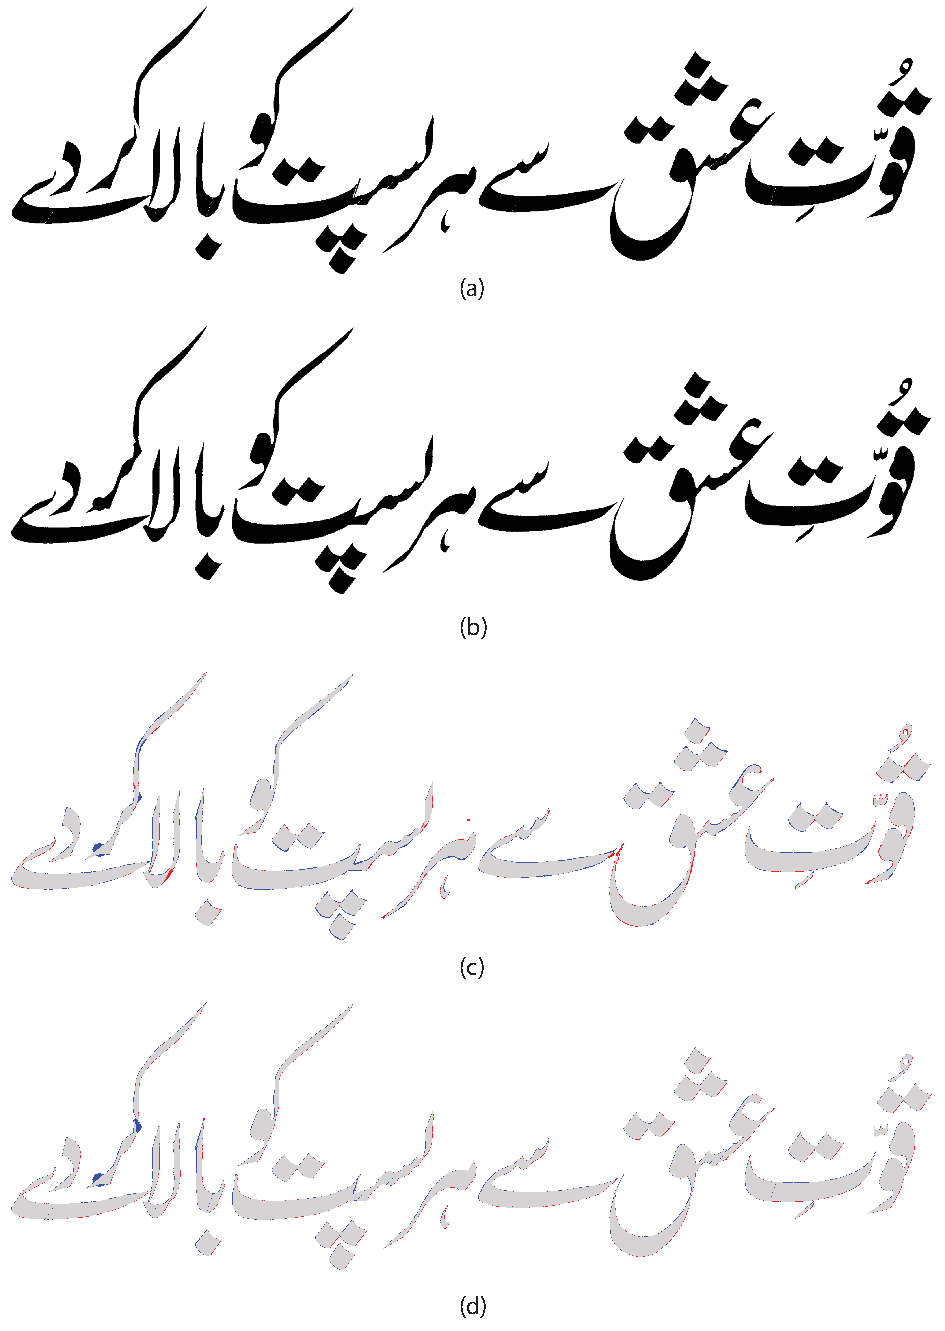
\includegraphics[width=0.8\textwidth]{../Images/Nastaleeq_Machined.pdf}
  \caption
  {
      Machined Nastaleeq sample by Gohar Qalam. (a) Rasterized rotating bezier spline for machining (b) Ink marks machined by a simulated robotic manipulator. (c) and (d) are differences between simulated ink mark and the rasterized photo and the processed original photo respectively. The red pixel indicate the portions that are missing in (c) but are present in the reference image and the blue ones show the missing pixels in reference but are present in the ink mark.
  }
\end{figure}

\begin{figure}[H]
  \centering
  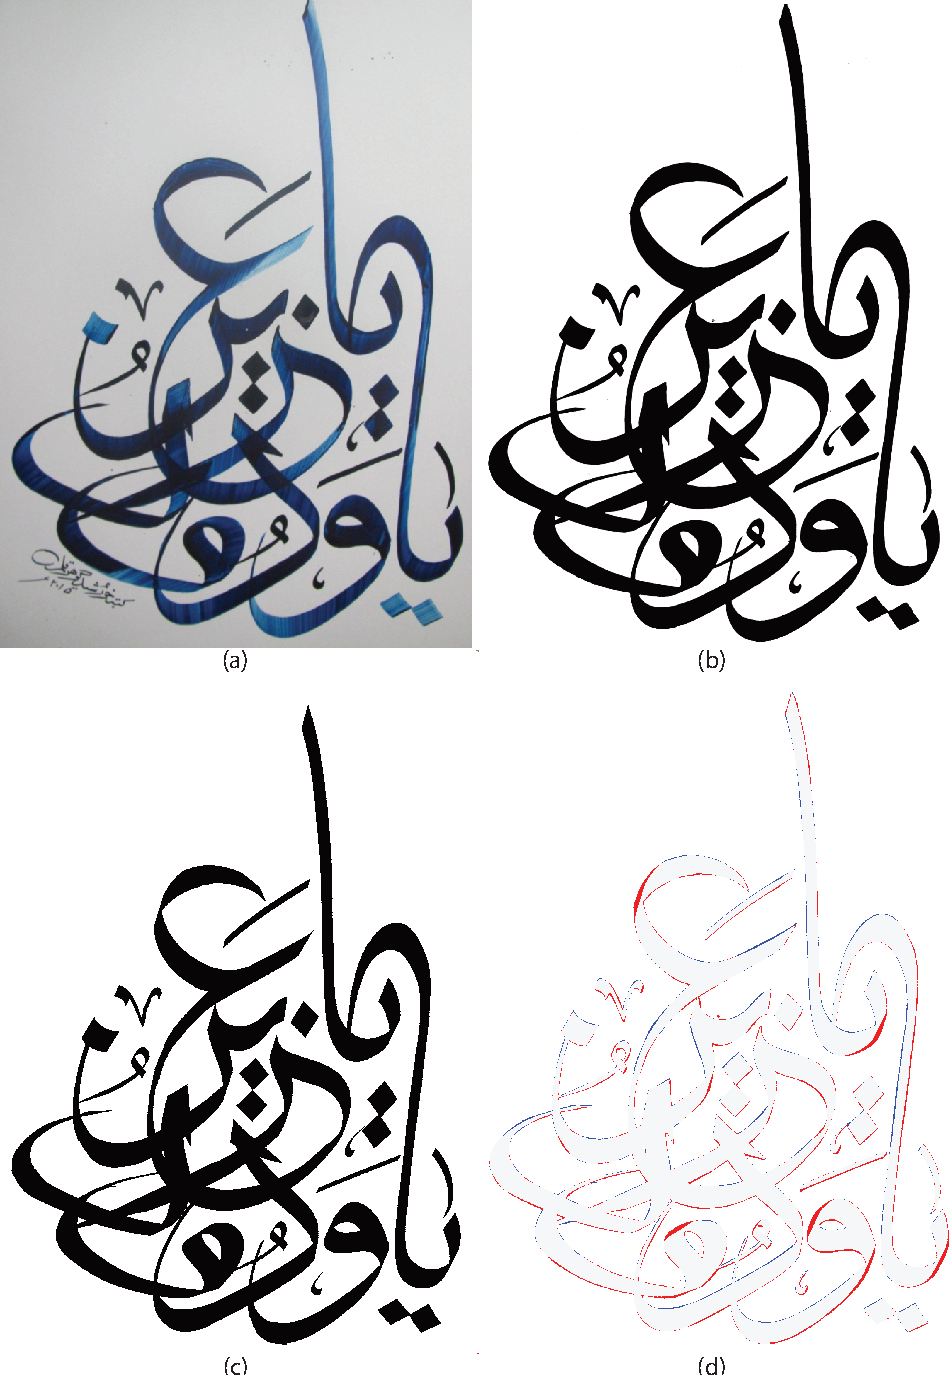
\includegraphics[width=0.8\textwidth]{../Images/Thuluth_Ink.pdf}
  \caption
  {
      Thuluth sample by Gohar Qalam. (a) Original calligraphy photo. (b) Original photo processed for analysis. (c) Traced rotating bezier spline ink. (d) Difference between (b) and (c). The red pixel indicate the portions that are missing in (c) but are present in (b) and the blue ones show the missing pixels in (b) but are present in (c).
  }
\end{figure}

\begin{figure}[H]
  \centering
  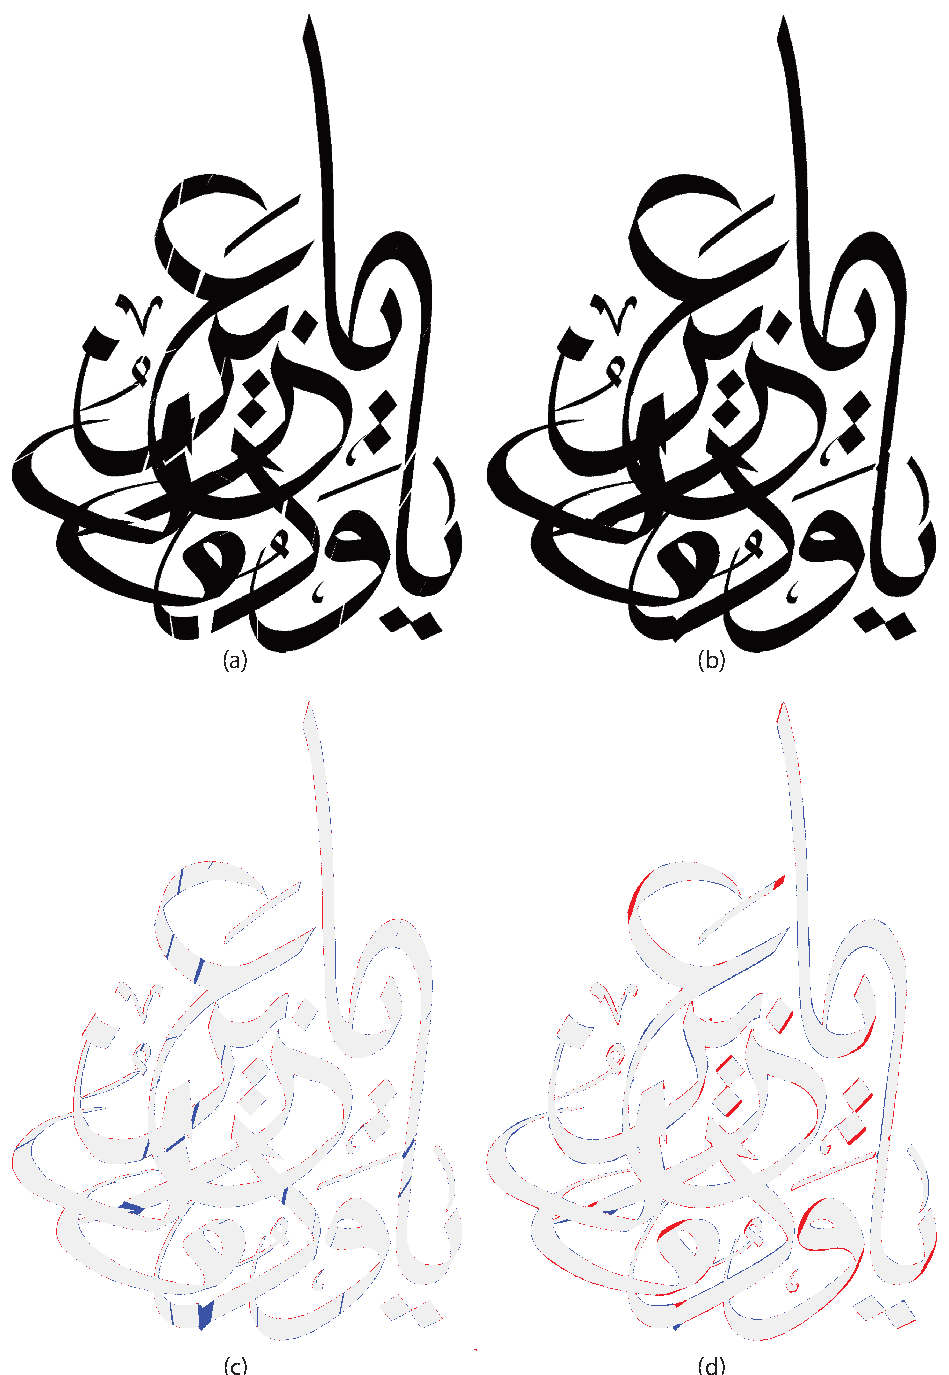
\includegraphics[width=0.8\textwidth]{../Images/Thuluth_Machined.pdf}
  \caption
  {
      Machined Thuluth sample by Gohar Qalam. (a) Rasterized rotating bezier spline for machining (b) Ink marks machined by a simulated robotic manipulator. (c) and (d) are differences between simulated ink mark and the rasterized photo and the processed original photo respectively. The red pixel indicate the portions that are missing in (c) but are present in the reference image and the blue ones show the missing pixels in reference but are present in the ink mark.
  }
\end{figure}
}
\section{Gregor -- A short user manual}\label{Appendix:Gregor}
\subsection{Features}
{
    From a developer's perspective there are some features that are either implemented inevitably along the way of implemented the essential features or the usability of these features outweighs the additional effort required for the implementation. For example, the developer would have to program at least one color that the view-port will use to visualize the splines. The effort required to just expose the color option to the user is negligible as compared to writing the rendering engine. Many such features were also made a part of Gregor.

    \begin{itemize}
    \item Toggling the visibility of curvature and rotation handles.
    \item Toggling the visibility of ink-marks.
    \item Changing the opacity and color ink-marks.
    \item Changing the viewing mode between editing and viewing.
    \item Grid snapping with an option to be toggled on or off.
    \item Changing the rendering mode of rotating bezier splines.
    \item Selecting, moving, deleting, hiding and enabling individual splines.
    \item Document explorer with thumbnails of every spline in the document.
    \item Importing splines into existing workspace
    \item Selecting, moving, deleting, hiding and enabling individual splines.
    \item Application menu to change options with keyboard shortcuts to most used menu items
    \end{itemize}
}
\subsection{Usage}
{
    The software can be used to create/trace new splines and also open up existing ones. The software uses Microsoft XML format to store data. While creating or editing a spline, the user adds more anchors by clicking on the desired position on the document. Anchors can be added to previous splines as well as the one under focus. Once a spline has been created, the user can change the thickness and color of the ink-mark and then fine tune the position of each anchor point to match the desired stroke. To trace the strokes of an existing document, the user can also load images on to the background of the document and resized and positioned at the desired position.

    Once some splines have been created, the user can choose to save the work as XML documents or be exported as images. The user can also compare the newly created artwork with the background images to analyze the false positive and false negative areas. The analysis tools can preview the difference and compute the number of pixels in each difference image.
}
\subsection{Interface}
{
    The view of the software is the spline editor with a detailed main menu as shown in Fig. \ref{Fig:GregorInterface}, document summary and a list of most commonly used toggle buttons. The application also provides some keyboard shortcuts for the most frequently used toggle options like changing the visibility of different elements and toggling the editing modes.

    The information a rotating spline contains is too much to be viewed simultaneously. The center point of the anchors, the curvature handles, twist handles, the curve, the inkmark and the background image, when displayed simultaneously is just chaotic. On top of that, when all of these elements are interactive, using a single mouse cursor to interface becomes a headache. This is why the application presents viewing and editing modes.
    \subsubsection{The Viewing Modes}
    {
        The viewing modes can be controlled using options (g1) through (g3) as shown in Fig.  \ref{Fig:GregorInterface}, the ``View'' menu (a2), or the keyboard shortcuts. There are essentially three modes of view.
        \begin{itemize}
          \item (g1) is ink and curve mode. In this mode, the splines curves and the selected handles will be shown alongwith the ink marks.
          \item (g2) is ink-only mode. In this mode, the curvature handle of the splines alongwith the anchors and the handles are hidden.
          \item (g3) is curve-only mode. The inkmark will be hidden in this mode and only the curve alongwith the selected handles will be visible.
        \end{itemize}
        it is obvious that only one mode can be activated at a moment and it can be selected either from the options (g1) through (g3) in Fig.  \ref{Fig:GregorInterface} or through the View menu. Instead of clicking on the toggle buttons, using the keyboard shortcuts can sometimes be even more convenient.
    }
    \subsubsection{The Editing Modes}
    {
        The editing models enable or disable the anchors, curvature handles and the twist handles. As shown in Fig. \ref{Fig:GregorInterface} (h1) through (h3), the editing mode toggle buttons can be used to enable or disable any of these handles. Just like the editing modes, these modes can also be controlled using the keyboard shortcuts. Unlike the viewing modes, however, these modes can be enabled all at a time. It must be noted that while in ink-only mode, none of the editing modes will have any effect of the usability of the editing handles.
    }

    \begin{figure}
      \centering
      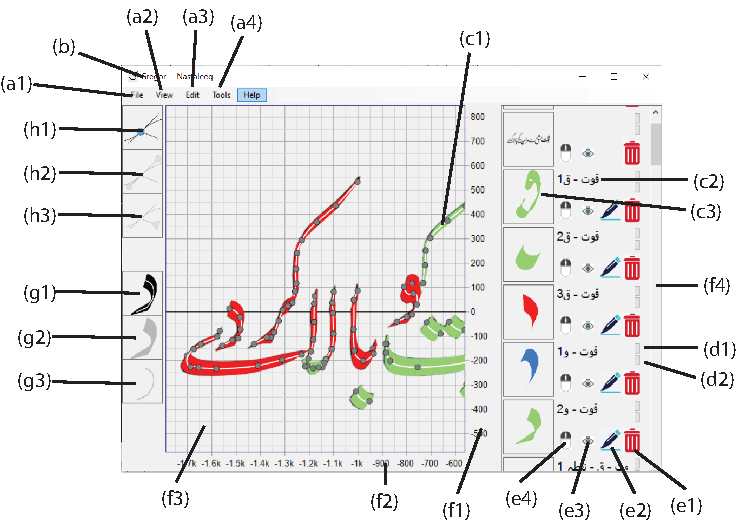
\includegraphics[width=0.9\textwidth]{../Images/GregorInterface.pdf}
      \caption{(a1-a4) The main menu options: (a1) Contains the options to open, save, import, export and clear splines and background images, (a2) enlists some viewing options; the ink viewing modes, visibility different elements of the workspace, visibility of background images, opacity of the ink-marks and rendering algorithm (a3) contains options related to editing on the workspace. It has the option to change the spline editing modes, the behaviour of left click on the workspace, and whether the splines can be dragged or not. (a4) has some analysis tools. (b) is the name of the currently open document. (c) is the main view of each spline in the document, (c2) and (c3) are the name of each spline element and its thumbnail respectively. (d1) and (d2) change the vertical order (z order) of the elements. While hovering the cursor over overlapping splines, the spline with higher position in the list will receive mouse event earlier. (e1), (e2), (e3) and (e4) are used to toggle editability, change visibility, modify color and thickness and delete the respective spline curve respectively. (f1) and (f2) are x and y axis of the workspace. (f3) is the main viewport. (f4) is the list of all the splines and images in the document. (g1) switches the view mode to both spline and inkmark, (g2) changes the viewing mode to ink only. (g3) changes the viewing mode to spline only. (h1), (h2) and (h3) toggle the visibility of center of anchor, curvature handle and the twist handle of the splines.
      } \label{Fig:GregorInterface}
    \end{figure}

}
\subsection{Modifying A Spline Curve}
{
    The application opens up an empty document by default. The first path one may choose to follow is to create new splines. This is done by adding new anchors. Anchors are added by simply clicking on an empty area of the screen. It must be noted that by default, the behaviour of the left mouse click must be switched from the Edit menu or using the keyboard shortcut to enable ``Add anchors using left mouse click''. Once an anchor has been added, adding a second anchor automatically creates a spline between the previously added anchor.
    \subsubsection{Starting a New Curve}
    {
        Since each click will append an anchor at the end of to the current spline, to break the curve and start a new one, some other procedure must be adopted. This can either be done by right clicking on an empty part of the document or toggling the ``Add anchors using left mouse click'' option off and quickly using the keyboard shortcut.
    }
    \subsubsection{Appending to a Previously Active Curve}
    {
        To append anchors at the end or the beginning of a previously active spline, simple click the center point of the first or the last center of anchor of the desired curve and it will be selected. Now, every new click will append to the selected curve just like before.
    }
    \subsubsection{Adding Anchors in the Middle}
    {
        Unfortunately adding anchor amid a curve is not a possibility yet. It would require an algorithm that can compute the nearest point on a curve from the mouse position that can show where the new anchor will be added. A work-around for now is to add anchors at the beginning or the end and soft the existing anchors inward until one of them reaches the required position.
    }
    \subsubsection{Simultaneous Curve Editing While Adding New Anchors}
    {
        It is usually very convenient to add an anchor while dragging the mouse cursor at the same time. This way, the software first adds an anchor just like it should on a mouse click but by dragging the cursor, instead of dragging the center of the newly added anchor, it drags the respective curvature handle instead. Creating new long strokes is very convenient this way. Please note that for this trick, the viewing mode must be showing the curve and both the centers and curvatures handles should be enabled.
    }
}
\subsection{Modifying an Ink-mark}
{
    \subsubsection{Adding an Ink-Mark}
    {
        Once a spline has been created with two or more anchors, the viewing mode can be switched to show ink and curve and the twist handle can be enabled while disabling the curvature handle. This will not convert the spline to a rotating curve unless it has been given a thickness. To change the thickness of a spline, simply click on it or the respective appearance in the document explorer as shown in Fig. \ref{Fig:AppearanceEditor} (e3). A curve appearance editor will pop up as shown in Fig. . Allowing to change both the broad edge thickness and the color of the ink-mark.

        \begin{figure}
          \centering
          \includegraphics[width=0.3\textwidth]{../Images/appearance editor.PNG}
          \caption{The curve appearance editor lets the user modify the color and broad edge thickness of the simulated pen} \label{Fig:AppearanceEditor}
        \end{figure}
    }
    \subsubsection{Modifying the twist/rotation}
    {
        Once the Ink-mark has some thickness, it will start to show up on the viewport as well. If the rotation handles are enabled, one can start dragging each rotation handle to start twisting the curve. The artist usually continuously switches between ink and curvature handles to keep modifying the final spline until they are satisfied with the final ink-marks.
    }
}
\subsection{Using Images}
{
    Images can be imported to an existing workspace by simply selecting the menu option File > Import > Image. One can choose to import an image directly from an image file or the clipboard if the user has already copied an image using a graphics editor like a photoshop or Microsoft Paint. To view it, the background images must also be enabled from the Edit menu. Once the image is visible, the user can select a discrete handle at the middle of the image to change the placement and an anchor at the top right corner to change the size, aspect ratio, mirroring and rotation of the image.
}
\subsection{Using the Document Explorer}
{
    In addition to shoing up in the viewport, all the images and splines also appear in the document explorer as shown in Fig. \ref{Fig:GregorInterface} (f4). Each item is represented by a multi-option control which shows some controls associated with the respective item.
    \begin{itemize}
      \item Fig. \ref{Fig:GregorInterface}(c3) is a normalized thumbnail of the respective item.
      \item One can change the name of each item using Fig. \ref{Fig:GregorInterface}(c2) which can come handy while dealing with multiple items which may look similar.
      \item (e1) will delete the respective item
      \item (e2) pops up the appearance menu of the respective curve
      \item (e3) toggles the visibility of the respective item
      \item (e4) toggles the editability of an item. A Disabled item can be viewed but not interacted with.
      \item (d1) and (d2) change the order of the z-order items in a document. A simple trick while moving an item in a very long list of items is to click once on the required move button and then instead of finding the relocated button again and clicking on it again, one can now choose to press the space bar or the enter button on the keyboard which will press the button again no matter where-ever it is.
    \end{itemize}

}
\subsection{Save, Load, Export}
{
    Once the user is satisfied with the artwork, they can save it using the File menu. Once saved, the user can save any further changes to the same file by simply using the well known save command ``Control + S'' or by using the Save option from the menu again. Once saved, the file can either be opened by using the Open option in the File menu or using the windows explorer. The saved files use an extension ``rbs''. The windows usually does not recognize this extension and will thus present a list of typical applications that can open it. Choose to browse for a custom application and point to the Gregor executable. The windows will not only open the file in Gregor but also remember this choice to open rbs files in the future.

    In addition to opening a file, a user can choose to import the curves contained in a file into an existing workspace, No current items will be cleared while importing a file.

    \subsubsection{Exporting Images}
    {
        Since the curves are vector data, one may still need to export this vector into a rasterized image to be used in various circumstances. A user can export the workspace in a pixel depth of their choice using the export option in the File menu. The export window as shown in Fig. \ref{Fig:ExportMenu} presents several options
        \begin{itemize}
          \item User can control whether to include the anchors and spline curves in the render
          \item The background images can also be exported alongwith the splines.
          \item A uniform color can be selected for the exported splines.
          \item The user can also specify the rendering algorithm for the ink-mark.
          \item Last but not the least, the user can specify a pixel density. By default, each unit on the grid will be considered one pixel. Specifying a pixel density of $100$~DPU specifies to generate one hundred pixels between one unit on the grid. It must be noted that while using too dense or too large images, the application might succumb to the memory load of the procedure. So it is wise to always save the data before attempting to export an image.
        \end{itemize}

        \begin{figure}
          \centering
          \includegraphics[width=0.9\textwidth]{../Images/ExportMenu.PNG}
          \caption{The curve appearance editor lets the user modify the color and broad edge thickness of the simulated pen} \label{Fig:ExportMenu}
        \end{figure}
    }
    \subsubsection{The File Format}
    {
        Gregor uses Microsoft XML format to save data. XML is primarily used to save text data. To pack images in it, the image is first converted into a hexadecimal list of byte data and represented as a very long string. It may inconvenience the user if they try to open it using a simple text editor which will show thousands of lines of gibberish hexadecimal bytes. One way to open the file as text is to open using an advanced raw text editor like Notepad++ or Sublime Text. These editors have the provision to collapse a certain node of an XML document, making the rest of the data more readable.
    }
}
\clearpage 
\end{document} 